\documentclass[notes]{beamer}          % print frame + notes
%\documentclass[notes=only]{beamer}     % only notes
%\documentclass{beamer}                 % only frames
 
\usecolortheme{beaver}

% Some commonly used packages
% (copied mainly from the Utrecht University theme: https://www.overleaf.com/project/5c900fa3bd9930036341116a)
\usepackage{ragged2e}  % `\justifying` text
\usepackage{booktabs}  % Tables
\usepackage{tabularx}
\usepackage{tikz}      % Diagrams
\usetikzlibrary{calc, shapes, backgrounds}
\usepackage{amsmath, amssymb, amsfonts, amsthm}
\usepackage{url}       % `\url`s
\usepackage{listings}  % Code listings
\usepackage{comment}  
\usepackage{mathtools}
\usepackage{graphicx}
\usepackage{subfig}
\usepackage{amsmath}

% Mainly math commands
\newcommand{\vect}[1]{\bm{#1}}
\usepackage{amsfonts}% to get the \mathbb alphabet
\newcommand{\field}[1]{\mathbb{#1}}
\newcommand{\C}{\field{C}}
\newcommand{\R}{\field{R}}
\newcommand{\norm}[1]{\left\lVert#1\right\rVert}
\newcommand{\argmin}{\operatornamewithlimits{argmin}}
\providecommand{\abs}[1]{\lvert#1\rvert}
\providecommand{\norm}[1]{\lVert#1\rVert}

% A variable used to exclude slides from the lecture version
\newif\iffull
%\fullfalse
\fulltrue

% Bibliography 
\usepackage[uniquename=init,giveninits=true,maxcitenames=1,style=authortitle-comp,backend=bibtex8]{biblatex}
%\bibliography{references}
\addbibresource{references.bib}


%Information to be included in the title page:
\title{Unsupervised learning}
\author{Federica Eduati}
\institute{Eindhoven University of Technology

Department of Biomedical Engineering}
\date{2020}
 
 
\begin{document}
 
\frame{\titlepage}
 
\section{Overview}

\begin{frame}
\frametitle{Learning goals}
At the end of this lecture you will:
\begin{itemize}
    \item Have a general understanding of what is unsupervised learning.
    \item Have a general understanding what is dimensionality reductions and some methods to do it.
    \item Have a general understanding of what is clustering and some methods to do it.
\end{itemize}

\vspace{5mm} 

Materials: 
\begin{itemize}
    \item Chapters 14 from \cite{elements}.
\end{itemize}

\end{frame}

\begin{frame}
\frametitle{Overview}
Topics of the lecture:
\begin{itemize}
    \item What is unsupervised learning?
    \item Methods for dimensionality reduction
    \begin{itemize}
    		\item Principal components analysis
    		\item t-SNE
    \end{itemize}
    \item Methods for clustering
    \begin{itemize}
    		\item K-means clustering
    		\item Hierarchical clustering
    	\end{itemize}
\end{itemize}

\vspace{5mm} 


\end{frame}

\section{Overview}




\section{General introduction}
\begin{frame}{Difference between supervised and unsupervised learning}
With both supervised and unsupervised learning we have a set of features $X_1, X_2, \dots, X_p$.

\vspace{5mm} 

\begin{itemize}
\item with \textbf{supervised learning} (or \textit{learning with a teacher}) we also have a variable $Y$ (a label).
\item with \textbf{unsupervised learning} (or \textit{learning without a teacher}) we don't have the label.
\end{itemize}

\end{frame}


\begin{frame}{Unsupervised learning}
The goal of \textbf{unsupervised learning} is to find similarities among observations based on the set of features.

\vspace{2mm} 

Two categories:
\begin{itemize}
   \item \textbf{Dimensionality reduction}: reduce the the dimensions of the input features to facilitate visualisation and identification of groups. Also used as preprocessing before applying supervised techniques.
   \item \textbf{Clustering}: techniques to discover unknown groups (clusters) in data.
\end{itemize}

\vspace{2mm} 

Compared to supervised learning:
\begin{itemize}
\item No need for labels (often difficult to retrieve)
\item No quantitative metrics to measure success; evaluation based on heuristic arguments.
\end{itemize}

\end{frame}



\begin{frame}{Principal Component Analysis (PCA)}
Idea: From the $p$ variables (often correlated), derive a smaller subset of variables that explain most of the variability of the original set.
\vspace{2mm} 
\begin{center}
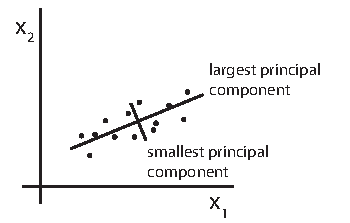
\includegraphics[height=4.2cm]{../figures/week_7/PrincipalComponetDrawing.pdf}  
\end{center}
\end{frame}

\begin{frame}{Principal Component Analysis (PCA)}
Starting from a set of features $X_1, X_2, \dots, X_p$, the \textit{first principal component} is the normalised linear combination of the features.

\begin{equation*}
	Z_1 =v_{11}X_1 + v_{21}X_2 + \dots + v_{p1}X_p
\end{equation*}

where $\sum_{j=1}^{p}v_{j1}^2=1$, and $v_{11}, v_{21}, \dots, v_{p1}$ are the \textit{loadings} of the first principal component and $v_1=(v_{11}, v_{21}, \dots, v_{p1}$) is the \textit{first principal component loading vector}.
\end{frame}

\begin{frame}{PCA computation - first principal component (PC1)}
We have our N observations $x_1, x_2,  \dots, x_N$, where each $x_i= (x_{i1}, x_{i2}, \dots, x_{ip})^T$, or in matrix form $\mathbf X$ of size $N \times p$.

\vspace{2mm} 

Since we are interested only in the variance we assume that each feature has 0 mean, i.e. $\mathbf X$  has columns with mean zero.

\vspace{2mm} 

We want to find the linear combination of the sample feature value:

\begin{equation*}
	z_{i1} =v_{11}x_{i1} + v_{21}x_{i2} + \dots + v_{p1}x_{ip}
\end{equation*}

with the largest sample variance, i.e.

\begin{equation*}
\max_{v_{11}, \dots, v_{p1}}  \{\frac{1}{N} \sum_{i=1}^N (\sum_{j=1}^p v_{j1}x_{ij})^2\} \text{     subject to   } \sum_{j=1}^{p}v_{j1}^2=1
\end{equation*}

Since each $x_{ij}$ has mean zero, also does $z_{ij}$. Hence we are maximising the sample variance of $Z_{1}$ which is $\frac{1}{N}\sum_{i=1}^N z_{i1}^2$.

\end{frame}

\begin{frame}{PCA computation - PC1 geometrical interpretation}
\begin{itemize}
\item The loading vector $v_1$ with elements $v_{11}, v_{21}, \dots, v_{p1}$ define the direction along which the data vary the most.
\item The projections of the N points $x_1, x_2, \dots, x_N$ onto this direction are the principal component scores $z_{11}, z_{21}, \dots, z_{N1}$.
\end{itemize}

\begin{center}
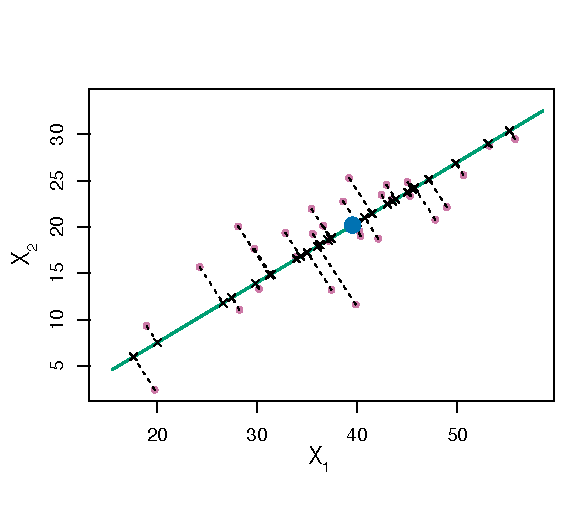
\includegraphics[height=5cm]{../figures/week_7/PCA_geometrical.pdf}  
\end{center}
\end{frame}

\begin{frame}{PCA computation - further principal components}
Now that we have the fist principal component $Z_1$ we want to find the \textit{second principal component}. $Z_2$. 

\vspace{2mm} 

$Z_2$ needs to be uncorrelated with $Z_1$. This is equivalent to constrain the direction of the loading vector $v_2$  is orthogonal to the direction of $v_1$.

\vspace{2mm} 
 
 Same for the following principal components.
 
 \begin{center}
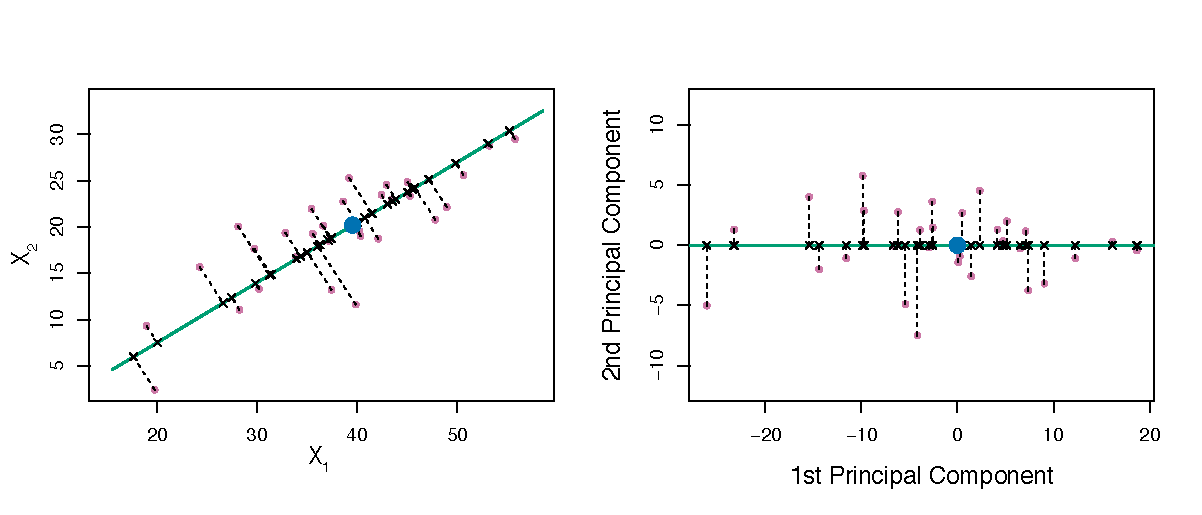
\includegraphics[height=4.2cm]{../figures/week_7/PCA_geometrical_part2.pdf}  
\end{center}
 

\end{frame}




\begin{frame}{PCA computation using SVD}
This optimisation problem can be solved via \textit{singular value decomposition} of the matrix $\mathbf X$:

\begin{equation*}
\mathbf X = \mathbf{UDV}^T
\end{equation*}
which is a unique decomposition such that (for $N \ge p$):

\begin{itemize}
\item $\mathbf{U}$ is a $N \times p$ orthogonal matrix ($\mathbf{U}^T\mathbf{U}=\mathbf{I}_p$)
\item $\mathbf{D}$ is a $p \times p$ diagonal matrix with $d_i \ge 0$ and $d_{i} \ge d_{i+1}$ known as the \textit{singular value}
\item $\mathbf{V}$ is a $p \times p$ orthogonal matrix ($\mathbf{V}^T\mathbf{V}=\mathbf{I}_p$)

\end{itemize}

The columns of $\mathbf{UD}$ are the \textit{principal components} of $\mathbf{X}$ ($PC1=u_{i1}d_1, PC2=u_{i2}d_2, \dots)$ and $\frac{d_{1}^2}{N}, \frac{d_{2}^2}{N}, \dots$ is the variance explained by each principal component.
\end{frame}

\begin{frame}{PCA example using images}
\begin{center}
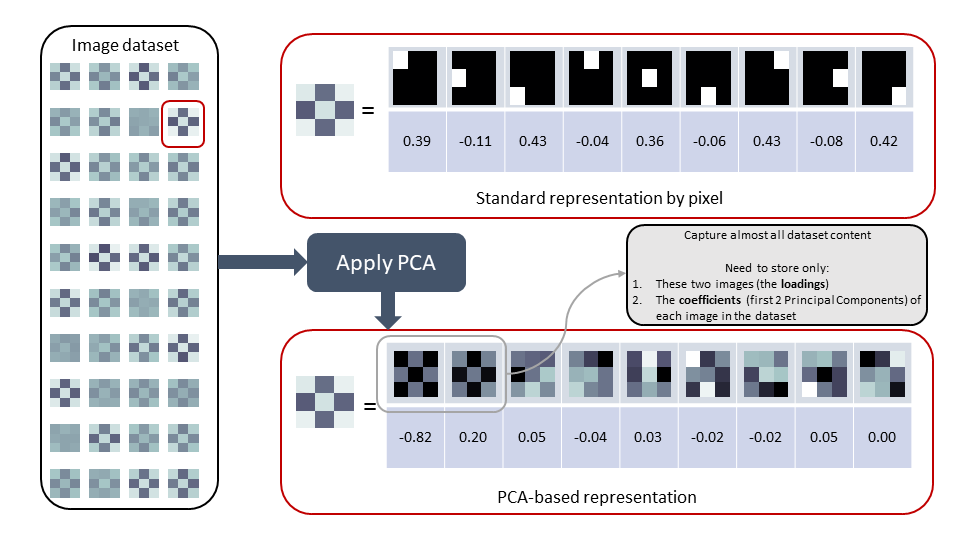
\includegraphics[height=6.2cm]{../figures/week_7/pca_image_example.png}  
\end{center}
\end{frame}


\begin{frame}{PCA example using GDSC dataset}
RNA expression data (244 genes) for 148 cell lines from four cancer types. Samples are \textit{a posteriori}  coloured by cancer type.
\begin{figure}
\minipage{0.45\textwidth}
  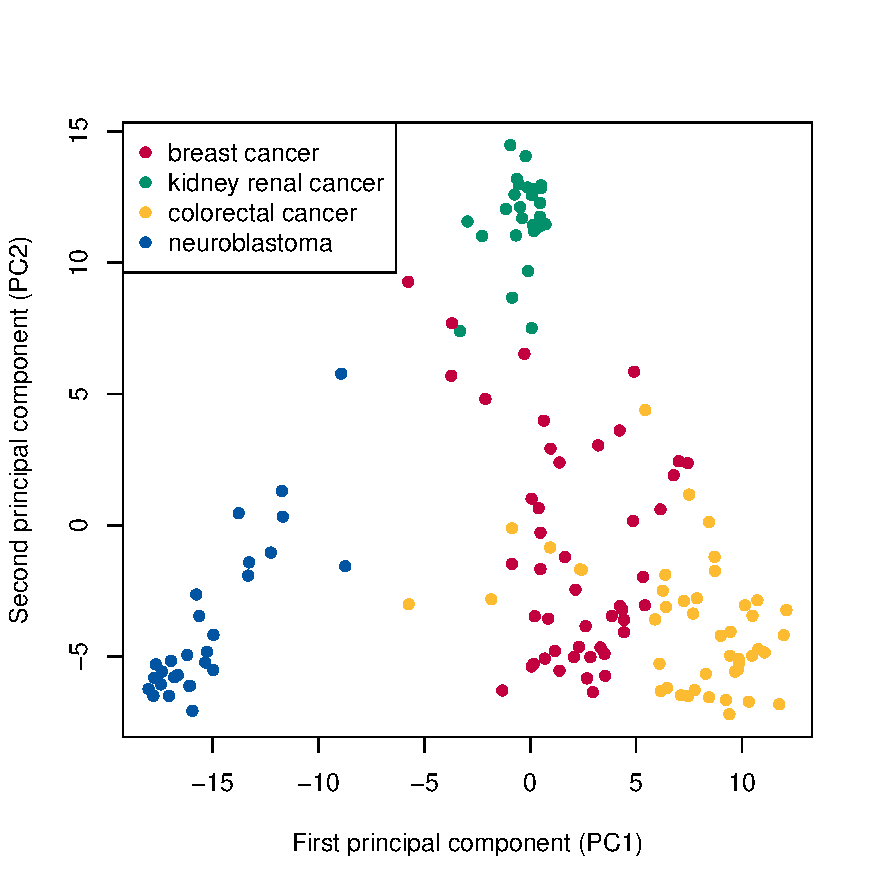
\includegraphics[width=\linewidth]{../figures/week_7/GDSC_2D_PC.pdf}  
\endminipage\hfill
\minipage{0.55\textwidth}
  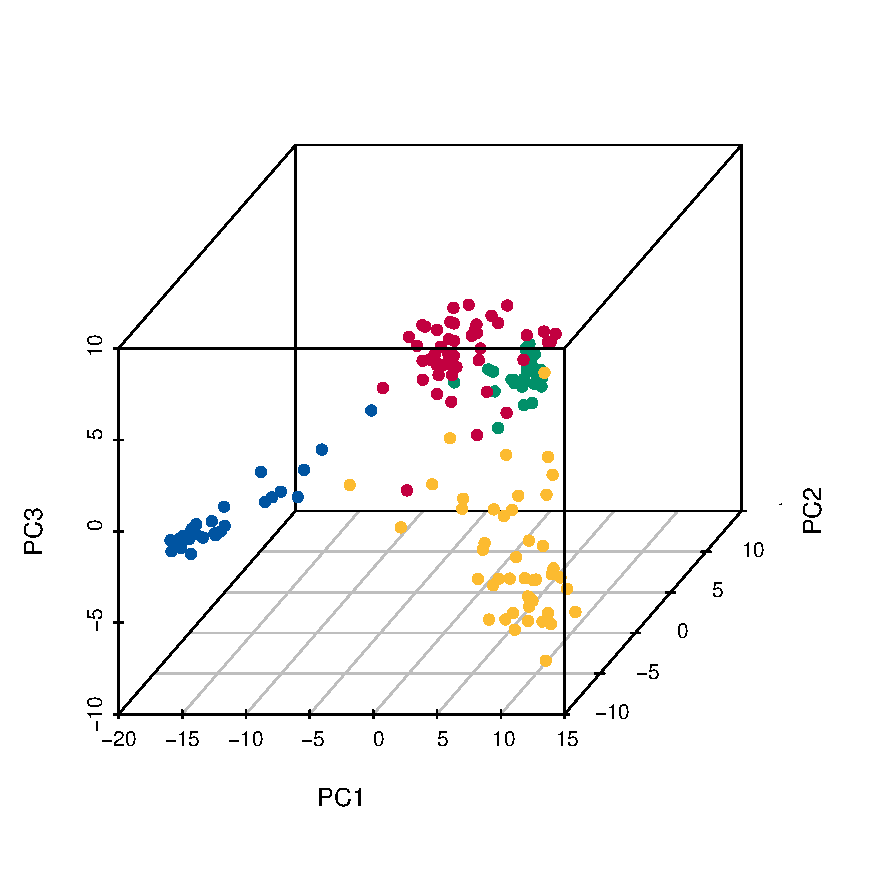
\includegraphics[width=\linewidth]{../figures/week_7/GDSC_3D_PC.pdf}  
\endminipage\hfill
\end{figure}
\end{frame}

\begin{frame}{PCA example using GDSC dataset - loads}
Loads of the first 3 principal components (only top 50 genes)
\begin{center}
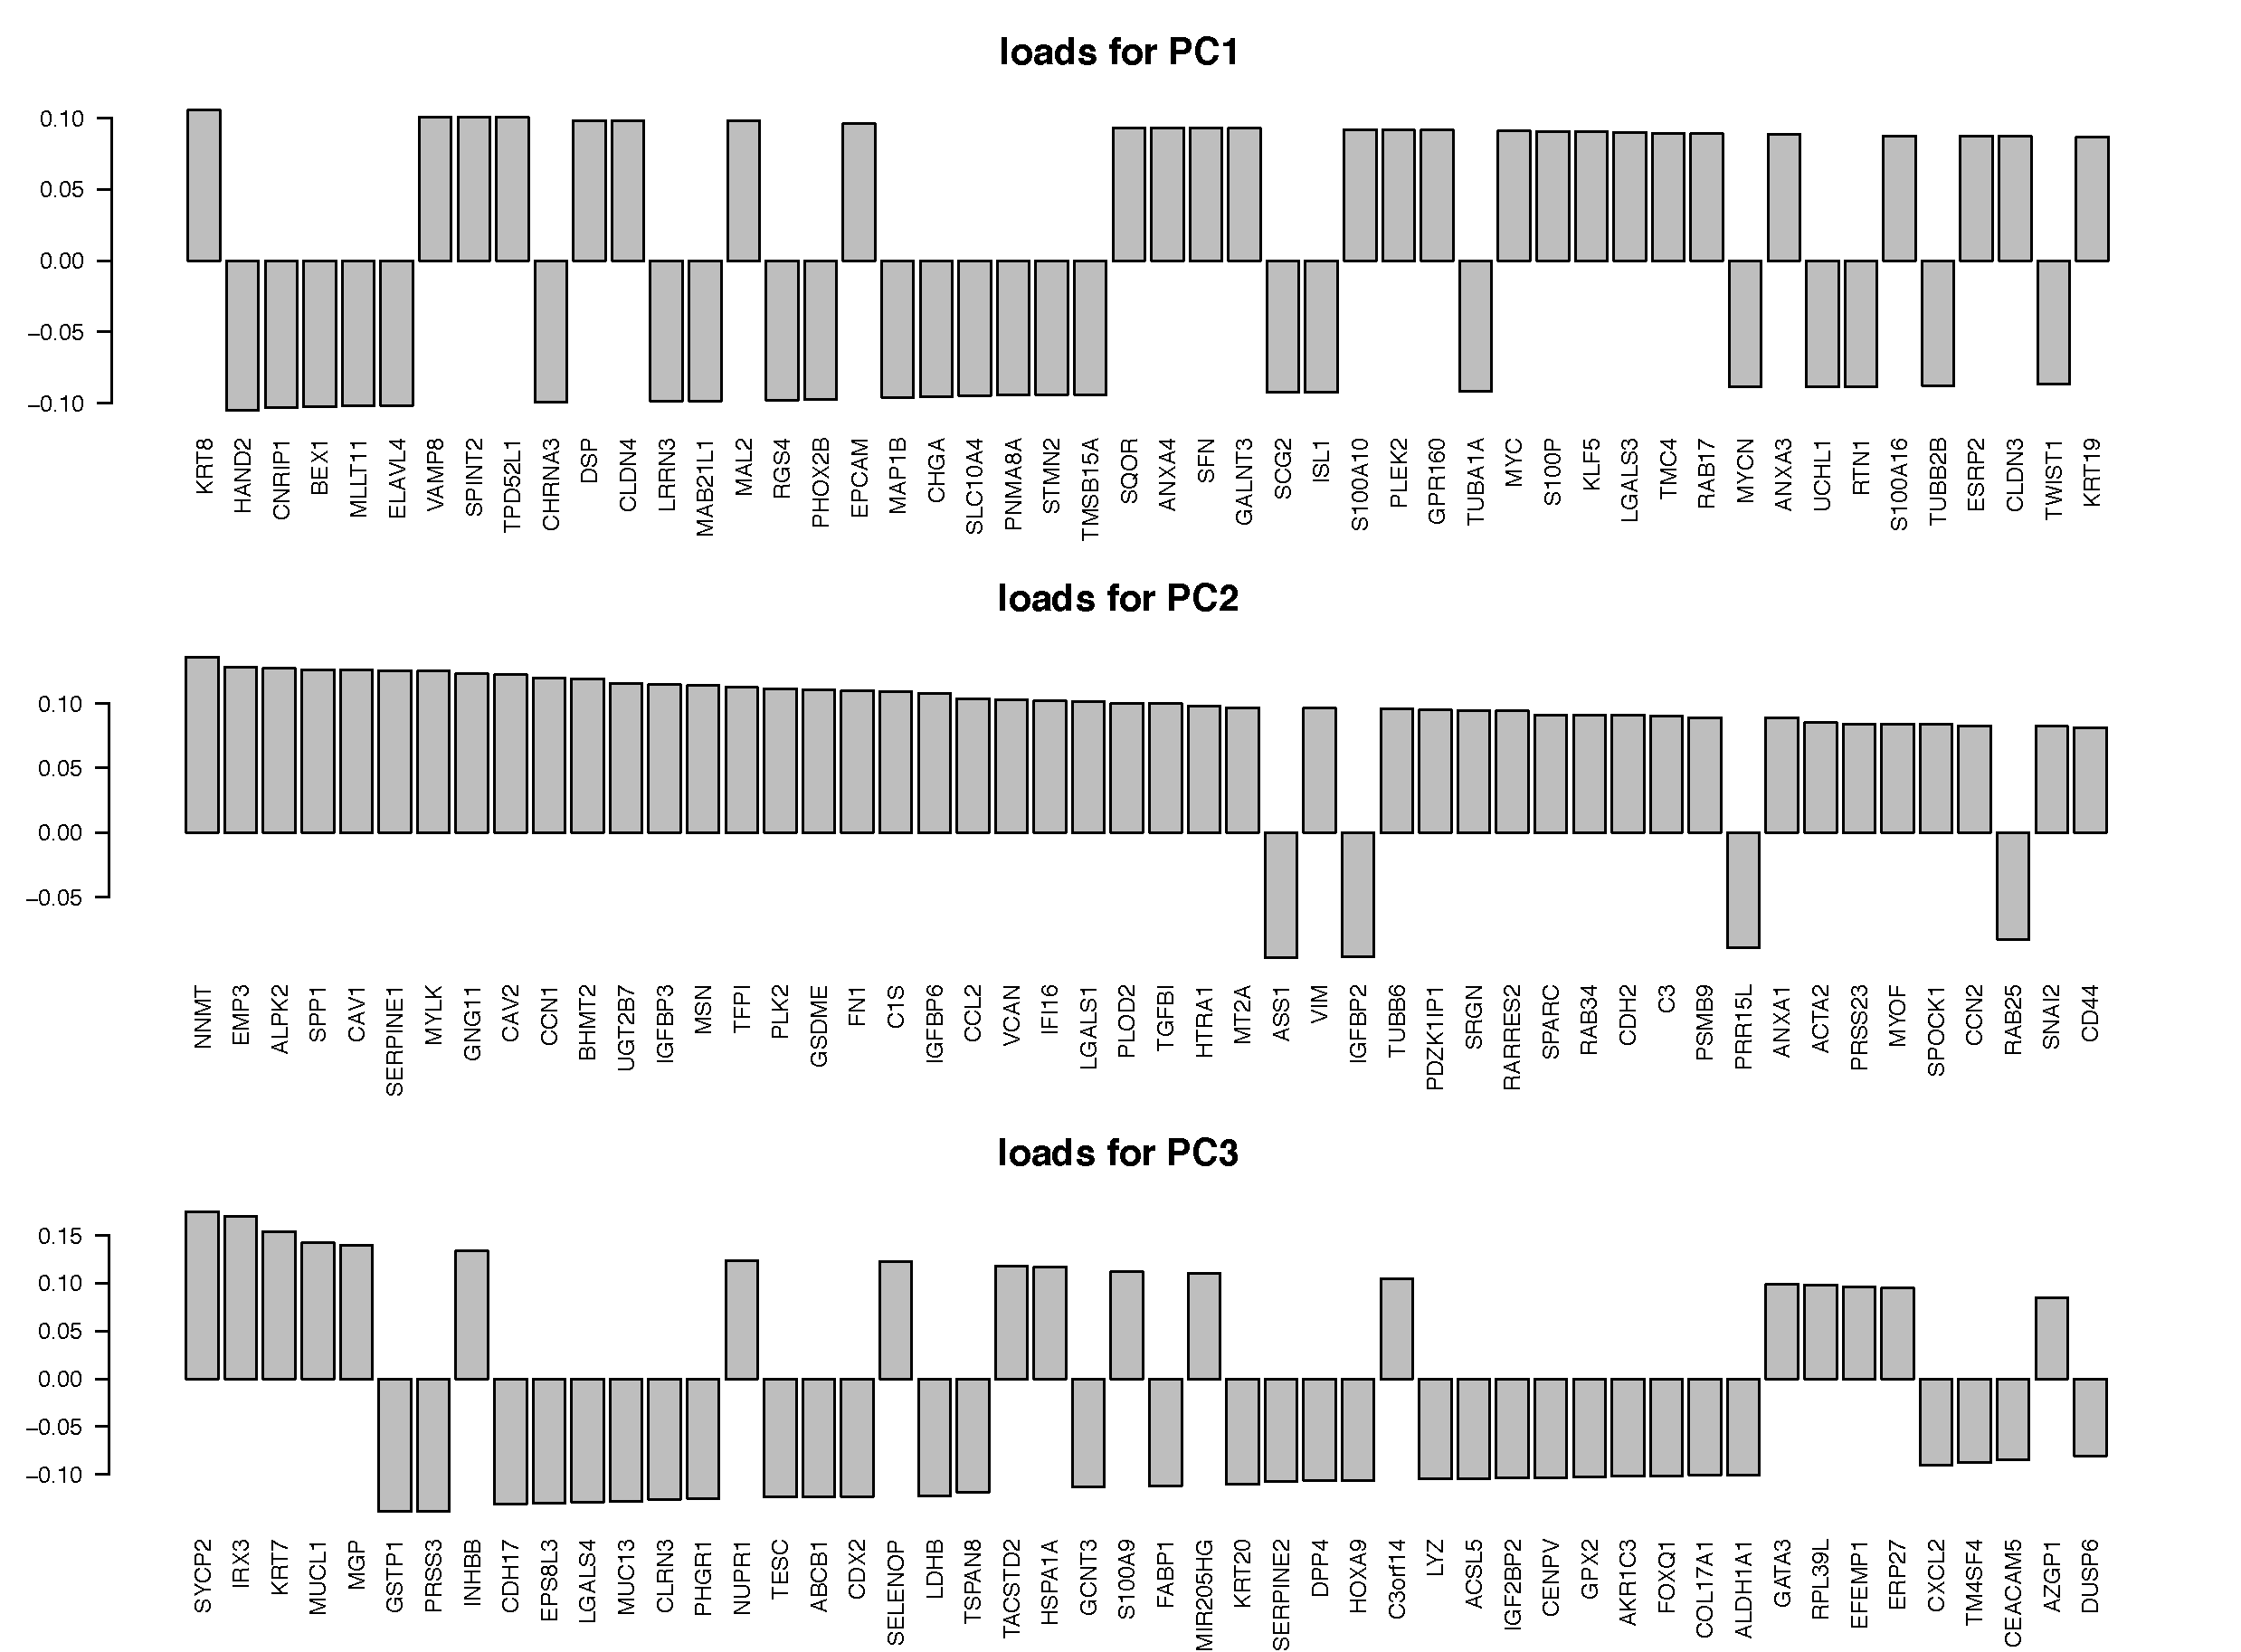
\includegraphics[height=7cm]{../figures/week_7/GDSC_loadsPC123.pdf}  
\end{center}
\end{frame}

\begin{frame}{PCA example using GDSC dataset - variance explained}
Variance explained by the principal components.
\begin{figure}
\minipage{0.50\textwidth}
  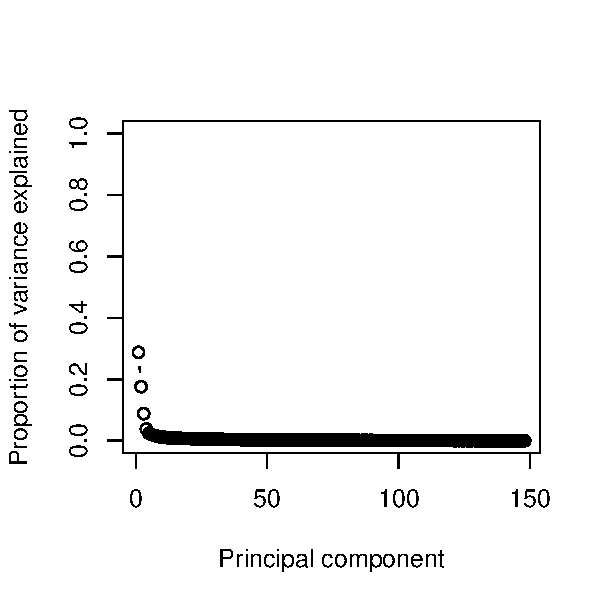
\includegraphics[width=\linewidth]{../figures/week_7/GDSC_PCA_variance.pdf}  
\endminipage\hfill
\minipage{0.50\textwidth}
  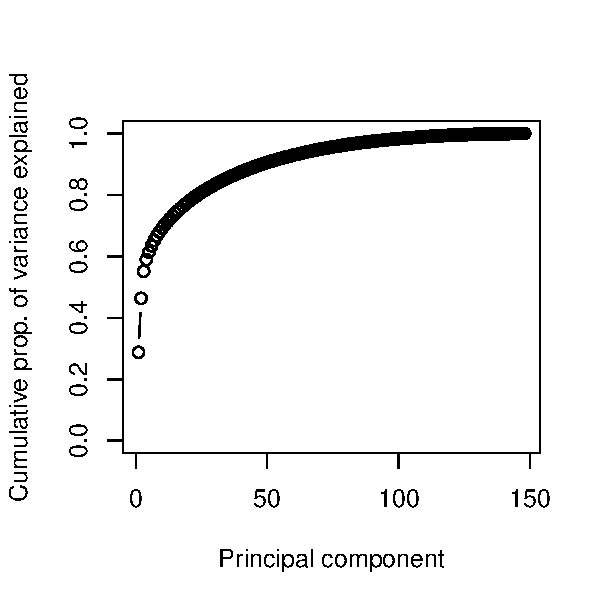
\includegraphics[width=\linewidth]{../figures/week_7/GDSC_PCA_cumul_variance.pdf}  
\endminipage\hfill
\end{figure}

Elbow in the "proportion of variance explained" plot can be used as a criteria to decide how many principal components to use.
\end{frame}

\begin{frame}{t-SNE}
\begin{itemize}
	\item PCA is a linear algorithm, i.e. principal components are linear combinations of the features.
	\item t-Distributed Stochastic Neighbor Embedding (t-SNE) is a non-linear techinque for dimensionality reduction.
	\item t-SNE works very well in high dimensional data.
	\item Cons: it is computationally demanding, it is stochastic and it is governed by hyperparameters.
\end{itemize}


\end{frame}

\begin{frame}{t-SNE computation}
\begin{itemize}
	\item Computes a measure of pairwise similarity in the original (multi-dimentional) feature space;
	\item Tries to minimise the difference between the similarity in the high-dimensional space and the similarity in a lower-dimensional space (typically 2 or 3 dimensions);
	\item The measure of similarity in the high- and low- dimensional space is different and this allows to visualise the clusters as more homogeneous.
	
	
\end{itemize}
\end{frame}

\begin{frame}{t-SNE example using GDSC data}
\begin{center}
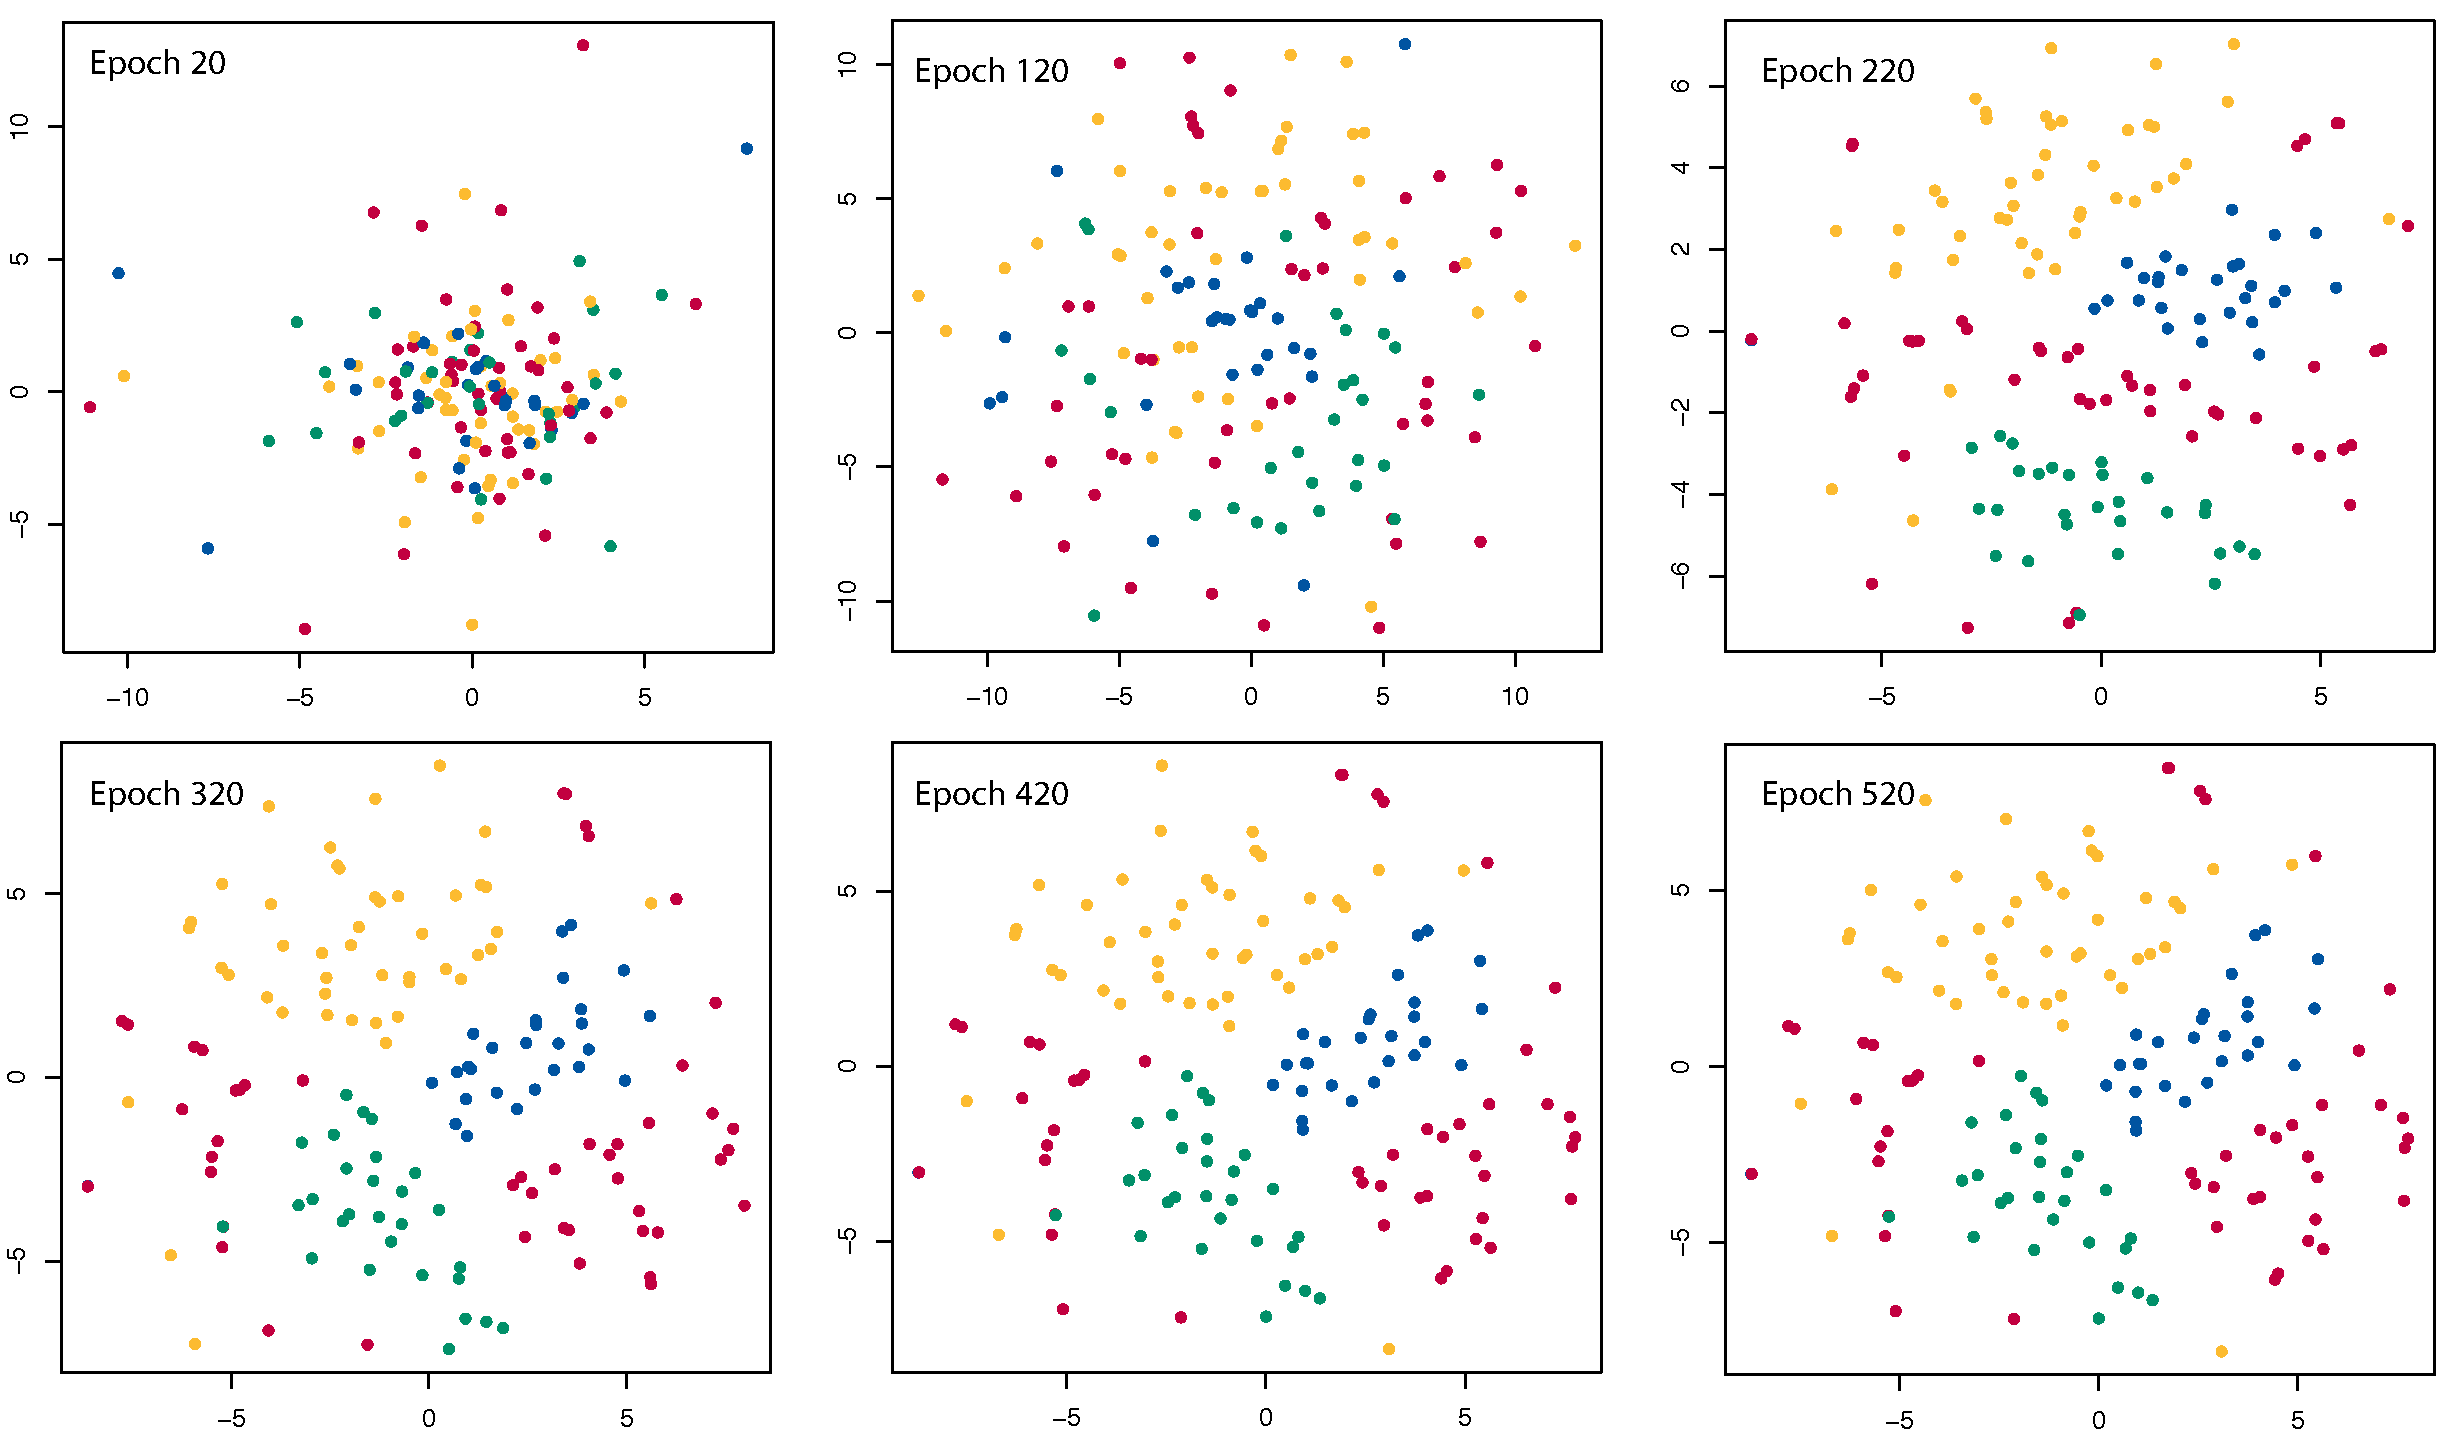
\includegraphics[height=6.2cm]{../figures/week_7/GDSC_tSNE.pdf}  
\end{center}
\end{frame}

\begin{frame}{Clustering}
\begin{itemize}

\item Aim: Group observations into subsets or \textit{clusters} or \textit{segments} so that observations within a cluster are more similar to each other than observations assigned to different cluster.
\item Requires a definition of \textit{similarity} or \textit{difference}.
\item This is similar to the definition of the cost function for supervised learning, the most appropriate definition of \textit{similarity} or \textit{difference} depend on the type of data.

\end{itemize}

\end{frame}

\begin{frame}{K-means clustering}
\begin{itemize}

\item Assign each observation $i \in \{1, 2, \dots, N \}$ to one cluster $k \in \{1, 2, \dots, K \}$.
\item $K$ need to be predefined, and $K < N$
\item This assignment correspond to a many-to-one mapping $k = C(i)$, which is an \textit{encoder} that assigns the $i$th observation to the $k$th cluster.
\item Each observation is assigned to one and only one cluster.

\end{itemize}

\end{frame}

\begin{frame}{K-means clustering}
We want to define the clusters so that similar points are in the same cluster and dissimilar points are in different clusters.

Defining $d_{i, i^\prime}=d(x_i, x_{i^\prime})$ as a measure of dissimilarity between a pair of observations $x_i$ and $x_{i^\prime}$, the total point scatter T is :

\begin{equation*}
	T = \frac{1}{2}  \sum_{i=1}^N \sum_{i^\prime=1}^N d_{i, i^\prime} = \frac{1}{2}  \sum_{k=1}^K \sum_{C(i)=k} (\sum_{C(i^\prime)=k} d_{i, i^\prime}  + \sum_{C(i) \neq k} d_{i, i^\prime})
\end{equation*}

Where:
\begin{itemize}
 \item $W(C) = \frac{1}{2} \sum_{k=1}^K \sum_{C(i)=k} \sum_{C(i^\prime)=k} d_{i, i^\prime}$ is the \textit{within-cluster} point scatter that we want to minimise
 \item $B(C) = \frac{1}{2} \sum_{k=1}^K \sum_{C(i)=k} \sum_{C(i^\prime) \neq k} d_{i, i^\prime}$ is the \textit{between-cluster} point scatter that we want to maximise
\end{itemize}

Minimising $W(C)$ or maximising $B(C)$ is equivalent.
\end{frame}

\begin{frame}{K-means clustering}
With K-means all variables has to be quantitative and we use the Eucledian distance as a measure of similarity:
\begin{equation*}
	d(x_i, x_{i^\prime}) = \sum_{j=1}^p (x_{ij} - x_{i^\prime j})^2 = \norm{x_{i} - x_{i^\prime} }^2
\end{equation*}

The within-point scatter can be written as:

\begin{equation*}
	W(C) = \frac{1}{2} \sum_{k=1}^K \sum_{C(i)=k} \sum_{C(i^\prime)=k} \norm{x_{i} - x_{i^\prime} }^2 = \sum_{k=1}^K N_k \sum_{C(i)=k}  \norm{x_{i} - \bar{x}_k }^2
\end{equation*}

where $N_k$ is the number of points in the $k$th cluster and $\bar{x}_k = (\bar{x}_{1k}, \dots, \bar{x}_{pk})$ is the mean vector associated with the $k$th cluster
\end{frame}

\begin{frame}{K-means clustering algorithm}
For high number of points $N$ it is infeasible to test all possible clustering assignments.

\vspace{2mm} 

We need \textit{iterative greedy descent} strategies to iteratively improve clustering assignments: 

\begin{enumerate}
 \item Randomly assign each observation to one cluster.
 \item Iterate the next two steps until cluster assignment stops changing
 \begin{enumerate}
 	\item For each cluster compute the mean vector $x_k$ (i.e. \textit{centroid})
 	\item Assign each observation to the cluster whose centroid is closest (based on Eucledian distance).
 \end{enumerate}
\end{enumerate}

\end{frame}

\begin{frame}{K-means iterations}
\begin{center}
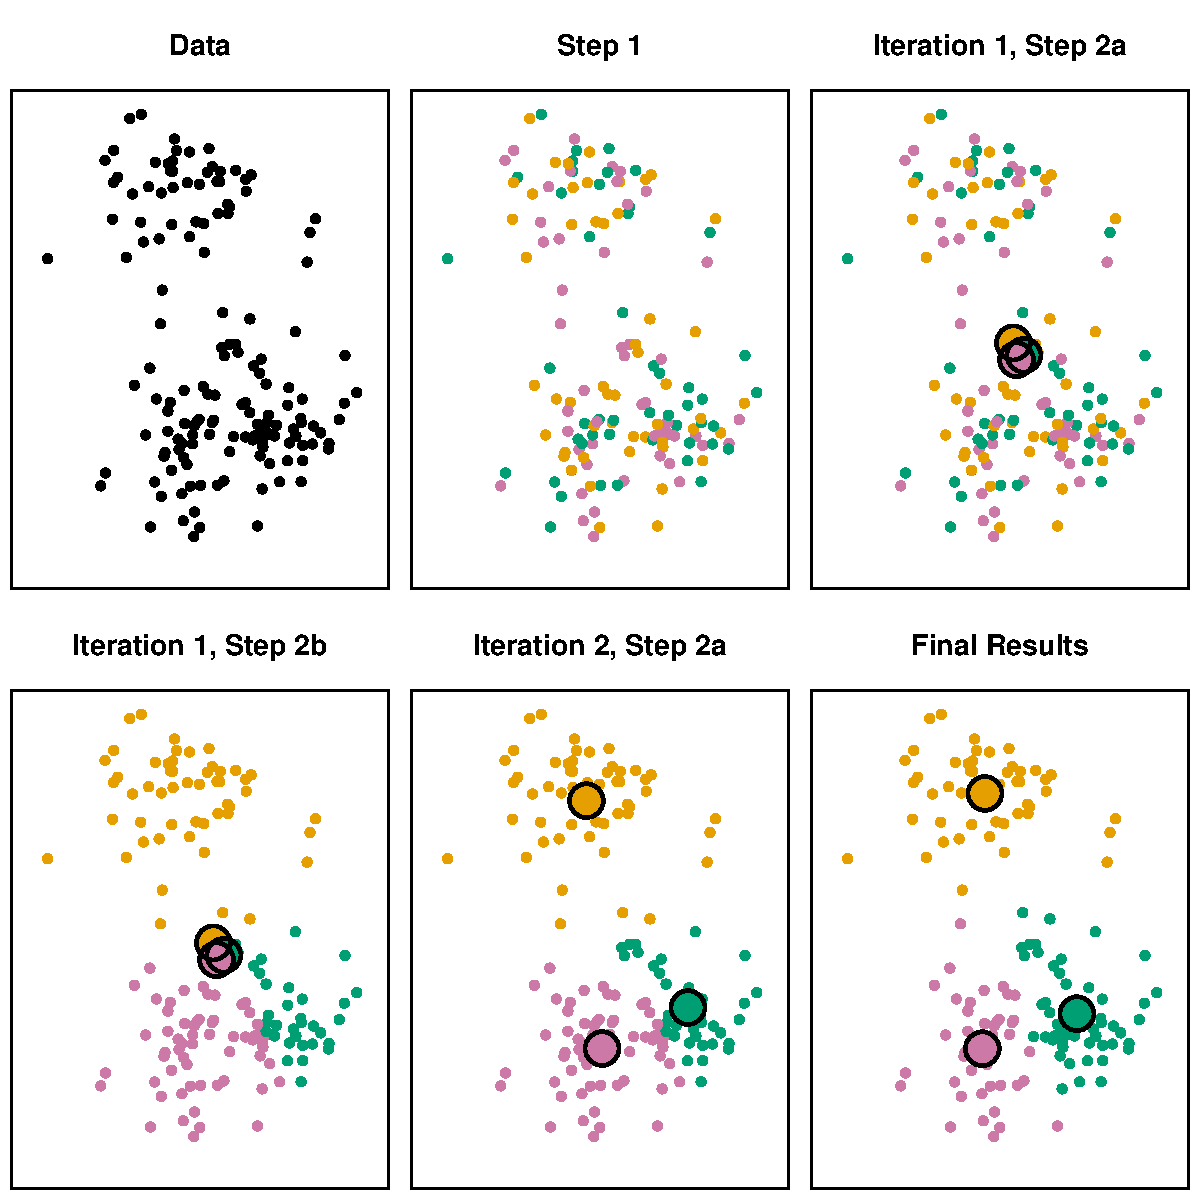
\includegraphics[height=7cm]{../figures/week_7/K-means_iterations.pdf}  
\end{center}
\end{frame}


\begin{frame}{K-means problems and solutions}
\begin{itemize}
 \item Problem: Does not guarantee the global minimum. Solution: we can check that no single switch of an observation to a different group decreases the objective function.
 \item Problem: Different random initialisation can provide different solutions. Solution: We can run it multiple times and select the solution with minimum objective function.
 \item We need to define the number of clusters.
\end{itemize}
\end{frame}

\begin{frame}{K-means example using GDSC data}

Compute K-means for different number of clusters and look at total within-cluster sum of squares for each clustering. 
\begin{center}
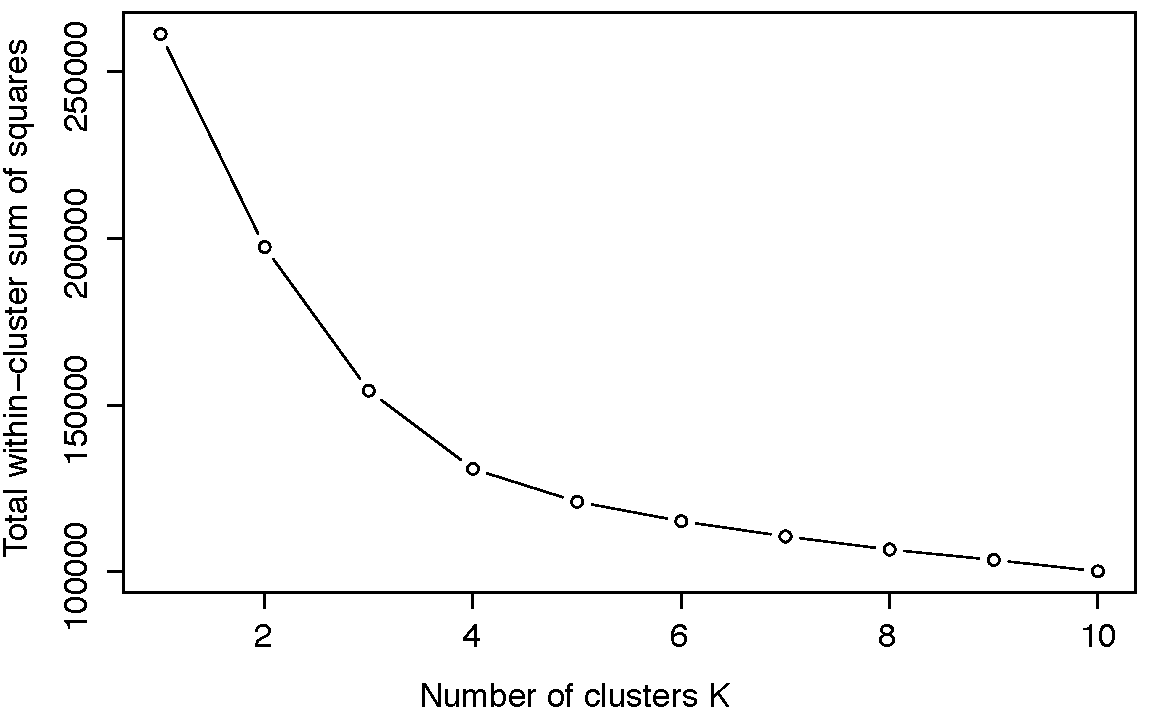
\includegraphics[height=5cm]{../figures/week_7/Kmeans_differentclustersize.pdf}  
\end{center}
Look at the elbow to define optimal number of cluster (not always possible).
\end{frame}

\begin{frame}{K-means example using GDSC data}
Number of cases of each cancer type (columns) in each cluster (rows), when using $K=4$.
\begin{center}
\begin{tabular}{ c | | c | c | c | c }
& breast & colorectal & kidney & neuroblastoma \\
\hline \hline
1 & 6 & 0 & 28 & 1 \\ 
2 & 41 & 7 & 0 & 0\\
3 & 0 & 37 & 0 & 0\\
4 & 0 & 1 & 0 & 27\\
\end{tabular}
\end{center}
\end{frame}



\begin{frame}{Hierarchical clustering}
\begin{itemize}
\item Differently from K-means, \textit{hierarchical clustering} does not require to specify a number of clusters.
\item It organises observations in a hierarchy, where clusters at each level of the hierarchy are created merging clusters at the next lower level.
\item The approach that we will see is \textit{bottom-up}
\begin{enumerate}
 \item It starts from the lowest level, where each observation is a singleton cluster.
 \item For $N-1$ steps it merges a selected pairs if clusters (i.e. the most similar) in a single cluster.
\end{enumerate}
\item This process can be visualized as a \textit{dendogram}
\end{itemize}
\end{frame}


\begin{frame}{Hierarchical clustering - Bottom-up approach }
\begin{center}
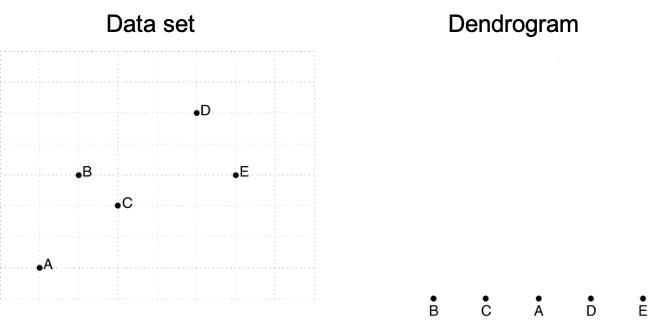
\includegraphics[height=5cm]{../figures/week_7/HierarchicalClustering_1.png}  
\end{center}
\end{frame}

\begin{frame}{Hierarchical clustering - Bottom-up approach - step 1}
\begin{center}
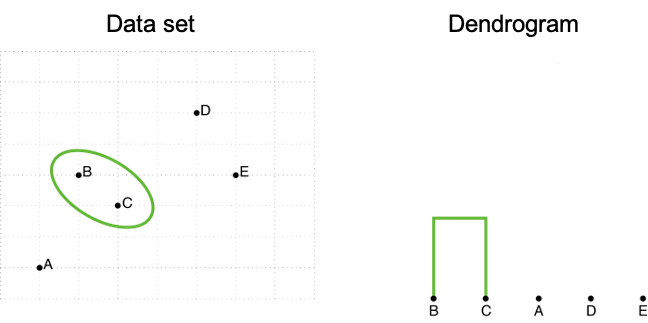
\includegraphics[height=5cm]{../figures/week_7/HierarchicalClustering_2.png}  
\end{center}
\end{frame}

\begin{frame}{Hierarchical clustering - Bottom-up approach - step 2}
\begin{center}
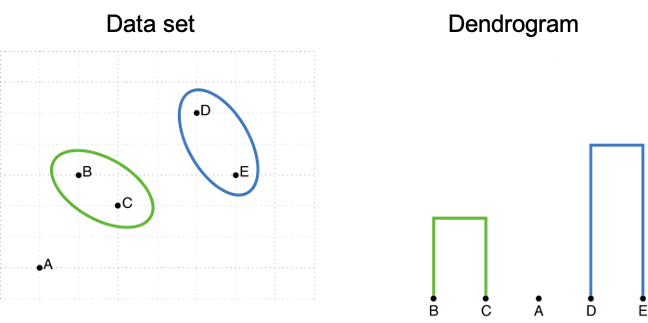
\includegraphics[height=5cm]{../figures/week_7/HierarchicalClustering_3.png}  
\end{center}
\end{frame}

\begin{frame}{Hierarchical clustering - Bottom-up approach - step 3}
\begin{center}
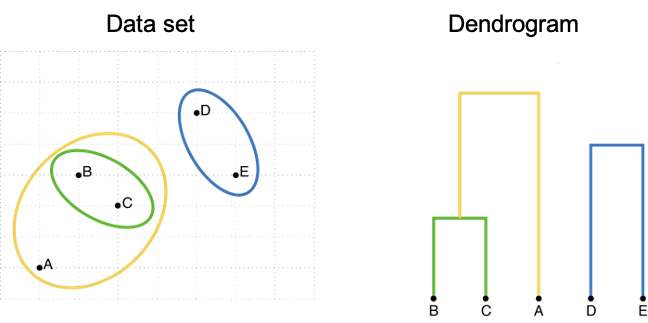
\includegraphics[height=5cm]{../figures/week_7/HierarchicalClustering_4.png}  
\end{center}
\end{frame}

\begin{frame}{Hierarchical clustering - Bottom-up approach - step 4}
\begin{center}
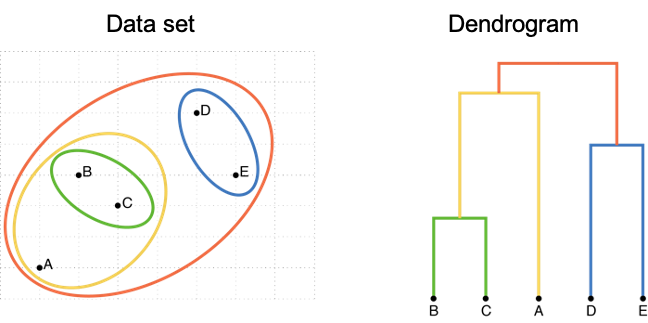
\includegraphics[height=5cm]{../figures/week_7/HierarchicalClustering_5.png}  
\end{center}
\end{frame}

\begin{frame}{Hierarchical clustering - Linkage}
How do we measure dissimilarity between two clusters (i.e. groups of observations)?
Consider two clusters $G$ and $H$, most used approaches are: 
\begin{itemize}
\item \textit{Single linkage}
\begin{equation*}
	d_{SL}(G, H) = \min_{i \in G, i^\prime \in H} d_{ii^\prime}
\end{equation*}
\item \textit{Complete linkage}
\begin{equation*}
	d_{CL}(G, H) = \max_{i \in G, i^\prime \in H} d_{ii^\prime}
\end{equation*}
\item \textit{Average linkage}
\begin{equation*}
	d_{CL}(G, H) = \frac{1}{N_G N_H} \sum_{i \in G} \sum_{i^\prime \in H}  d_{ii^\prime}
\end{equation*}
\end{itemize}
\end{frame}

\begin{frame}{Hierarchical clustering - Dissimilarity measure}
How do we measure dissimilarity between two points?
\begin{itemize}
\item  Most commonly used is Euclidean distance.
\item Another used metric is correlation (of observations across features).
\end{itemize}
\end{frame}


\begin{frame}{Hierarchical clustering - How to interpret a dendogram}
\begin{itemize}
\item Branches' height is proportional to the similarity between nodes.
\begin{itemize}
\item Observations that fuse at the bottom of the dendogram are similar to each other.
\item Observations that fuse at the top of the dendogram are different from each other.
\end{itemize}
\item We can cut the dendogram at a certain hight to obtain clusters.
\end{itemize}
\end{frame}

\begin{frame}{Hierarchical clustering - How to obtain clusters}
\begin{center}
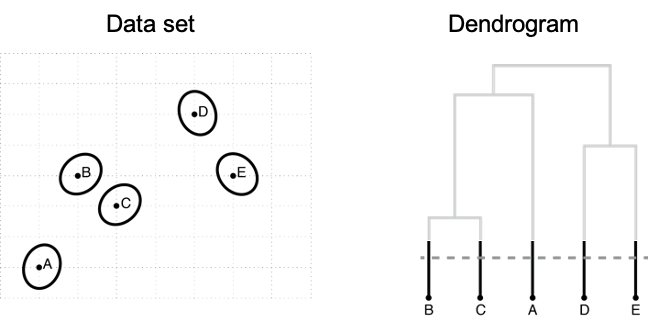
\includegraphics[height=5cm]{../figures/week_7/HierarchicalClustering_clusters_1.png}  
\end{center}
\end{frame}

\begin{frame}{Hierarchical clustering - How to obtain clusters}
\begin{center}
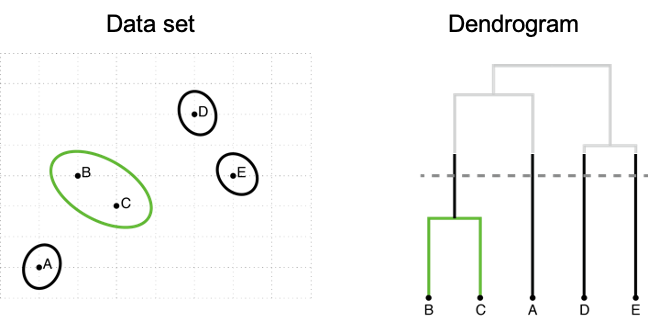
\includegraphics[height=5cm]{../figures/week_7/HierarchicalClustering_clusters_2.png}  
\end{center}
\end{frame}

\begin{frame}{Hierarchical clustering - How to obtain clusters}
\begin{center}
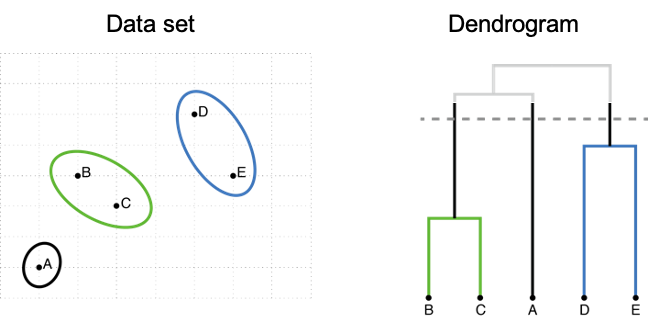
\includegraphics[height=5cm]{../figures/week_7/HierarchicalClustering_clusters_3.png}  
\end{center}
\end{frame}

\begin{frame}{Hierarchical clustering - How to obtain clusters}
\begin{center}
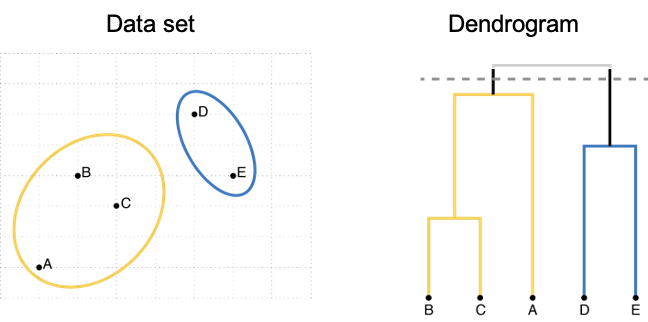
\includegraphics[height=5cm]{../figures/week_7/HierarchicalClustering_clusters_4.png}  
\end{center}
\end{frame}

\begin{frame}{Hierarchical clustering - How to obtain clusters}
\begin{center}
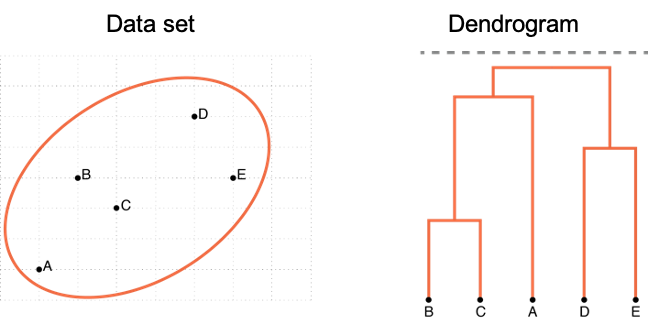
\includegraphics[height=5cm]{../figures/week_7/HierarchicalClustering_clusters_5.png}  
\end{center}
\end{frame}

\begin{frame}{Hierarchical clustering - examples with GDSC data}
Clustering using complete linkage for cluster similarity and Eucledian distance as observations similarity metric.
\begin{center}
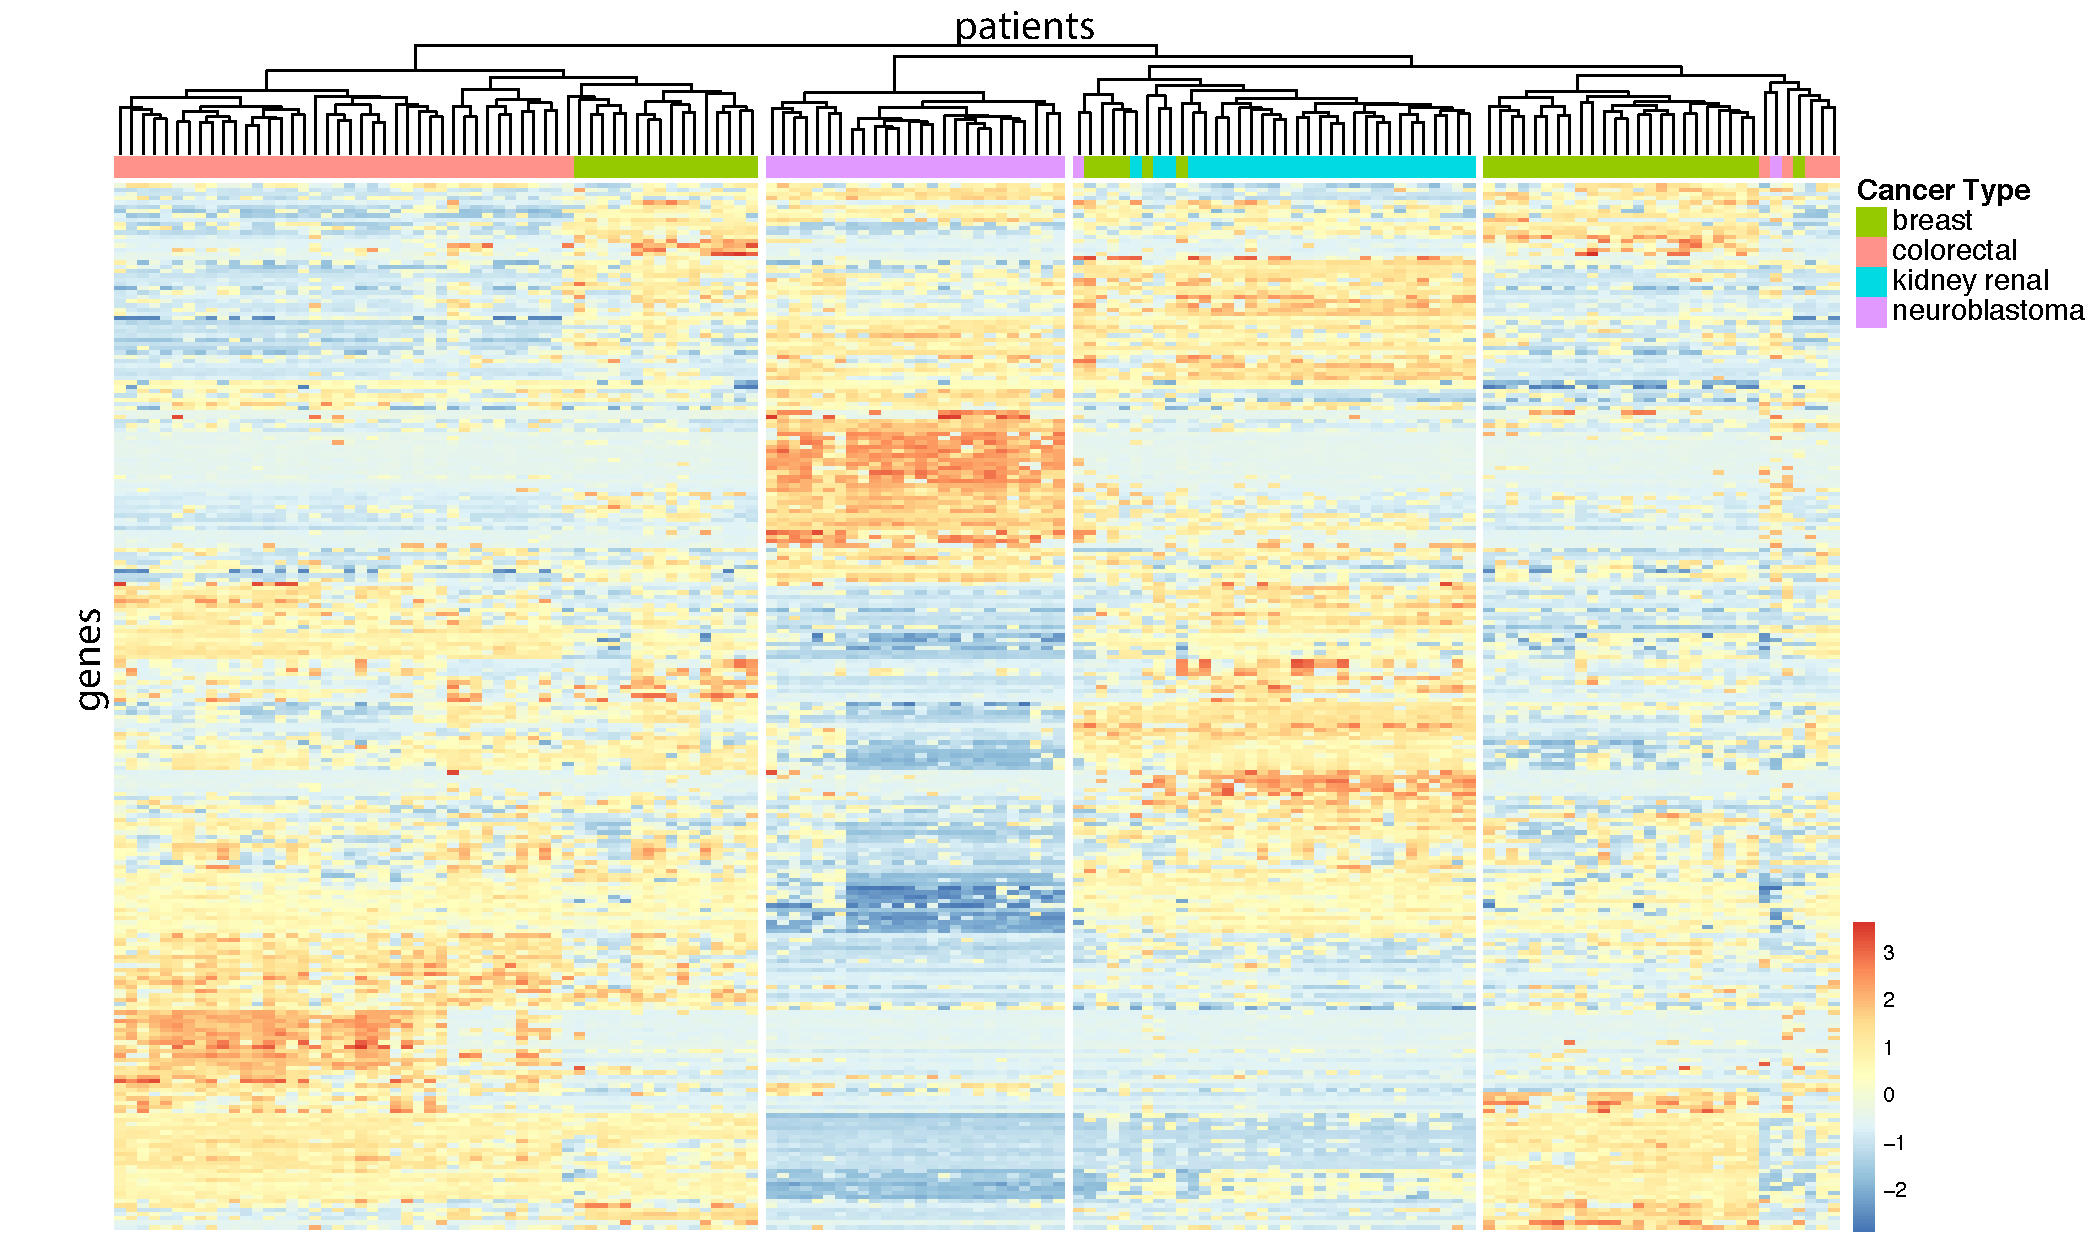
\includegraphics[height=6.2cm]{../figures/week_7/GDSC_heatmap_complete.pdf}  
\end{center}
\end{frame}

\begin{frame}{Hierarchical clustering - examples with GDSC data}
Clustering using single linkage for cluster similarity and Eucledian distance as observations similarity metric.\begin{center}
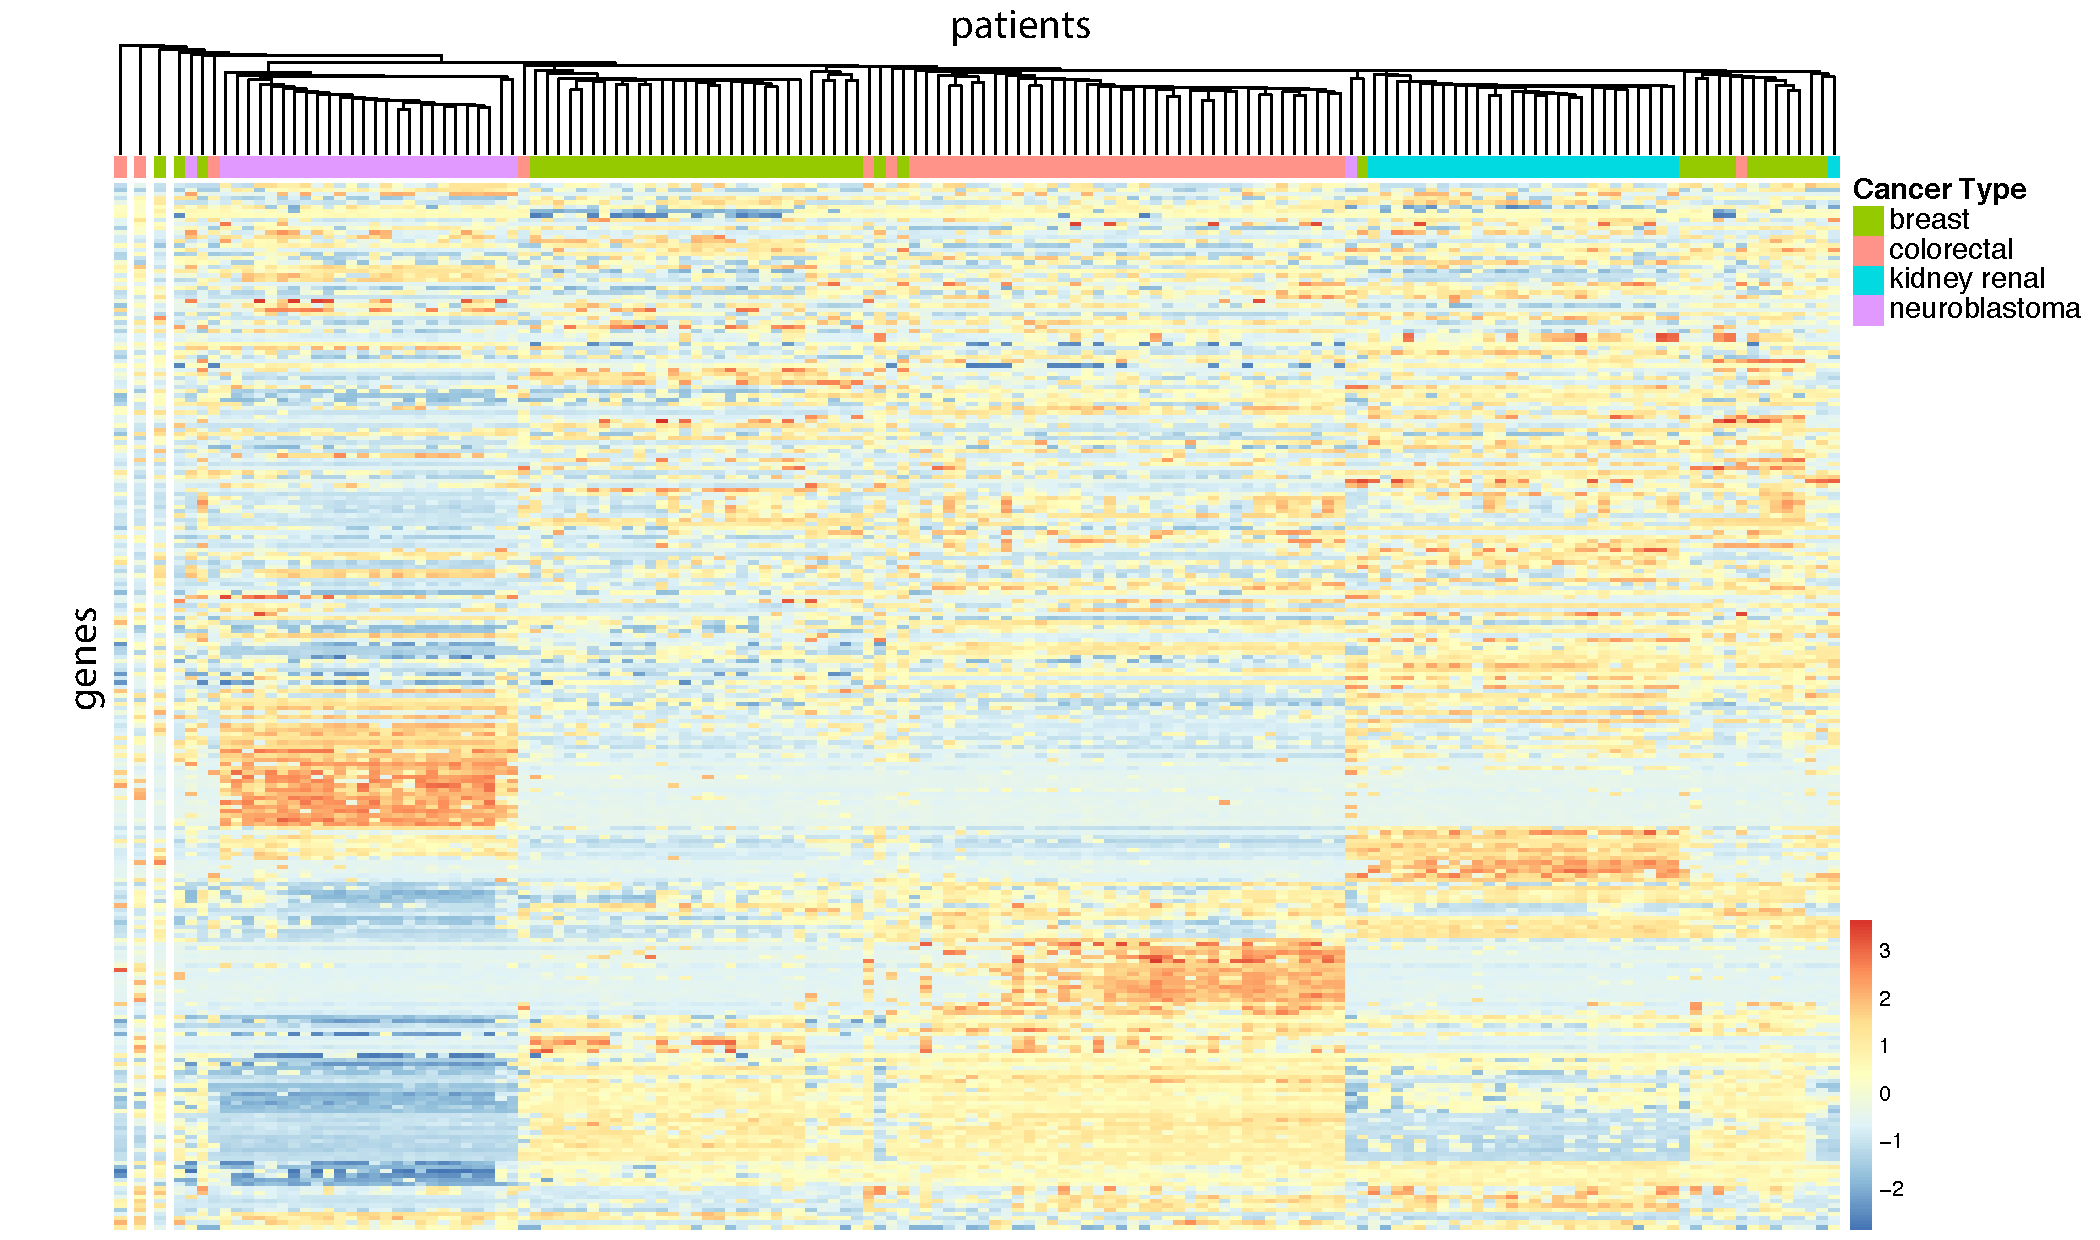
\includegraphics[height=6.2cm]{../figures/week_7/GDSC_heatmap_single.pdf}  
\end{center}
\end{frame}

\begin{frame}{Hierarchical clustering - examples with GDSC data}
Clustering using complete linkage for cluster similarity and correlation as observations similarity metric.
\begin{center}
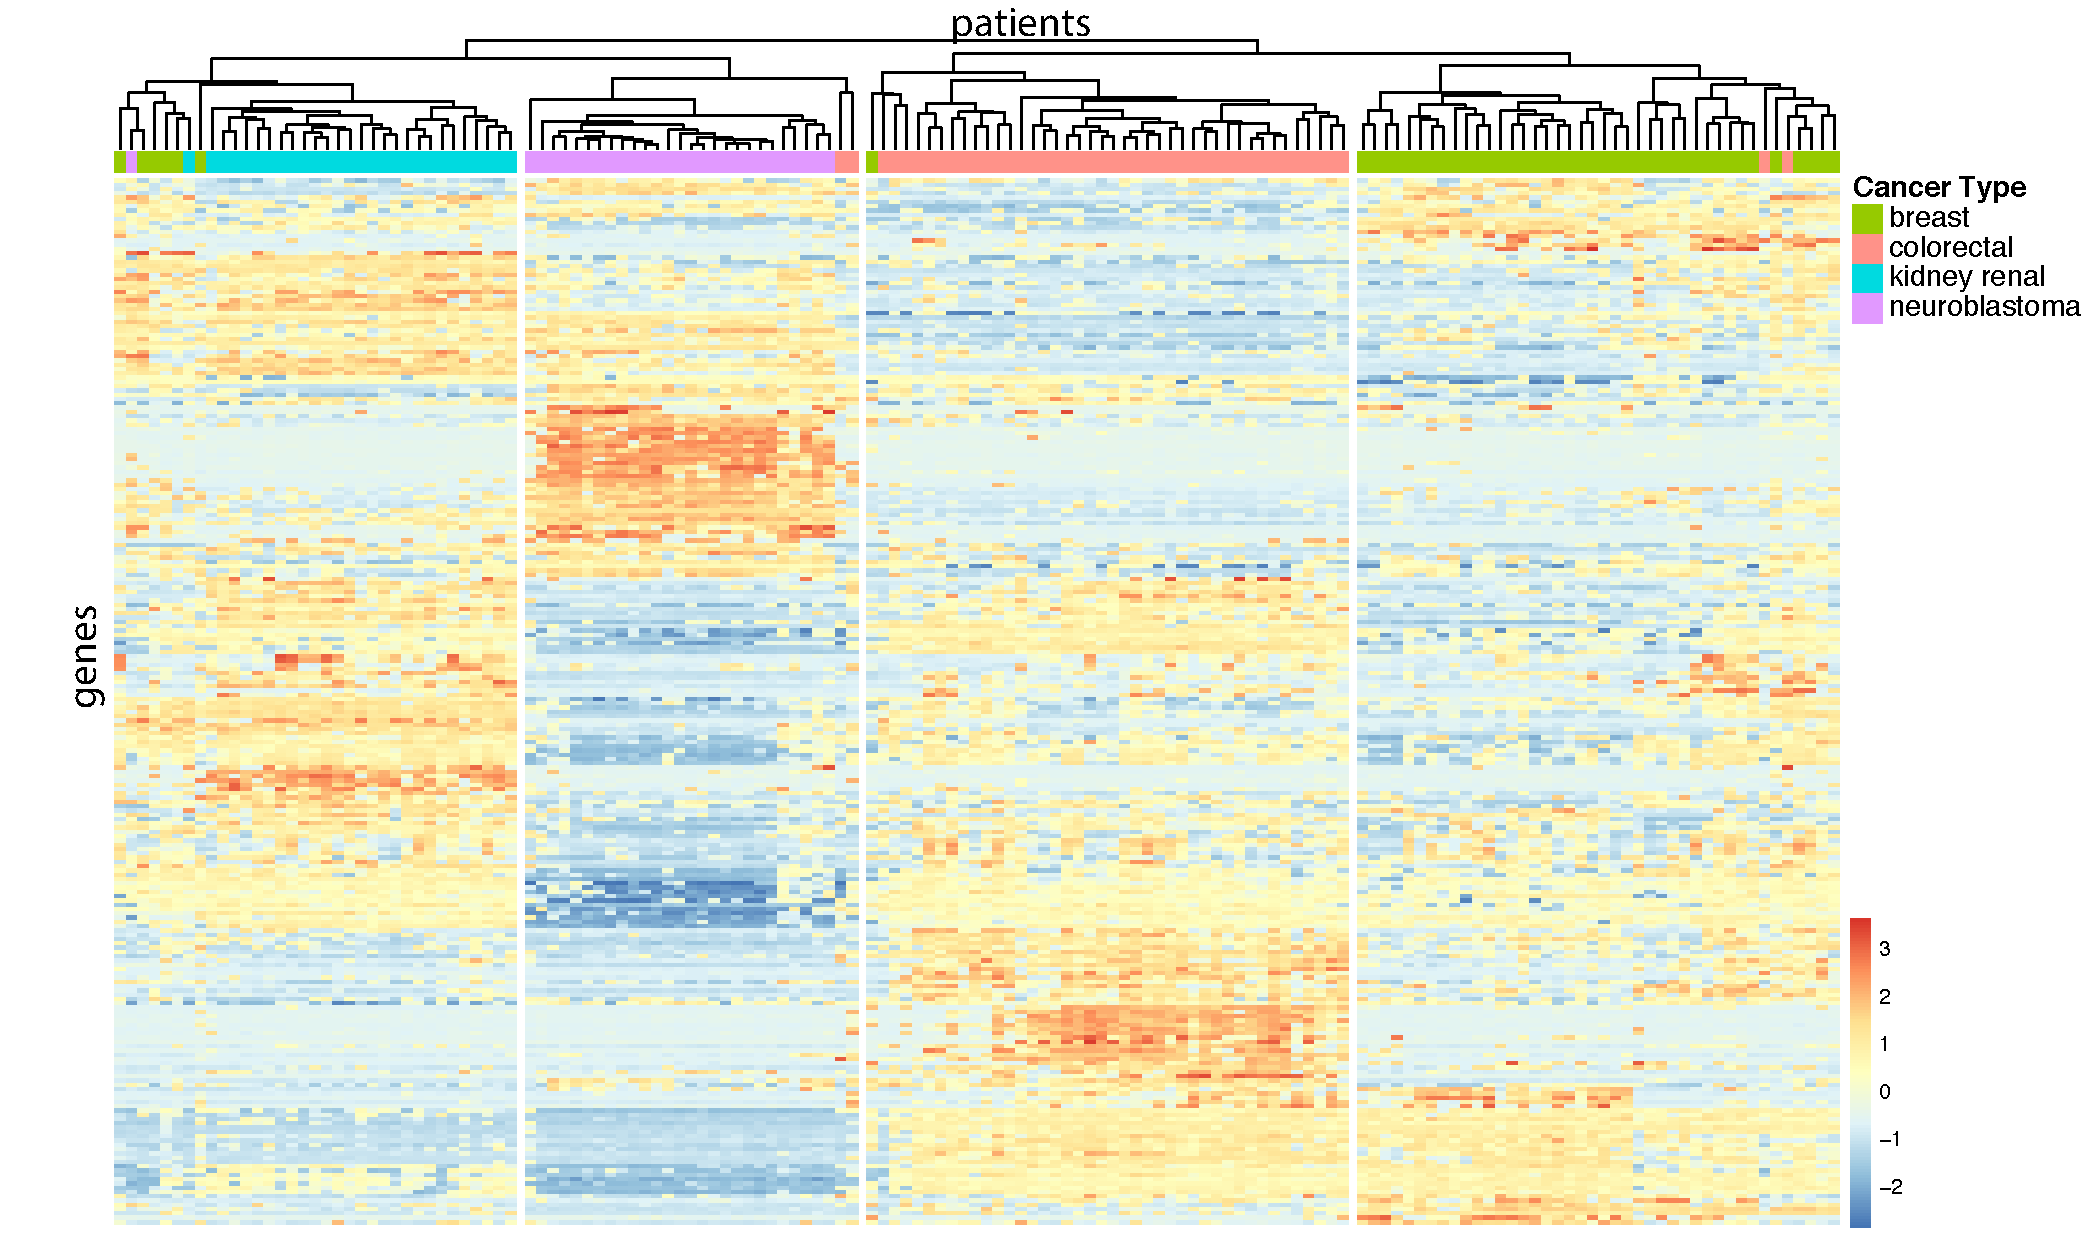
\includegraphics[height=6.2cm]{../figures/week_7/GDSC_heatmap_correlation.pdf}  
\end{center}
\end{frame}

\begin{frame}{Conclusions}
\begin{itemize}
\item Unsupervised learning is useful to find inherent patterns in data. 
\item It does not use/require labels on data. 
\item No gold standard to assess performances.
\item Used a lot for data exploration and/or as first step to then apply supervised learning.
\item Active field of research, essential to explore increasingly available high-dimensional data.
\end{itemize}
\end{frame}




\begin{frame}{References}
\begin{itemize}
\item The figures showing geometrical interpretation of PCA and iterations of K-means are taken from "An Introduction to Statistical Learning, with applications in R"  (Springer, 2013) with permission from the authors: G. James, D. Witten, T. Hastie and R. Tibshirani 
\end{itemize}
\printbibliography
\end{frame}
\end{document}